\documentclass[10pt,a4paper]{article}
\usepackage[utf8]{inputenc}
\usepackage{amsmath}
\usepackage{amsfonts}
\usepackage{amssymb}
\usepackage{geometry}
\usepackage{verbatim}
\usepackage{enumerate}
\usepackage{fancyvrb}
\usepackage{graphicx}
\usepackage{tikz}
\usetikzlibrary{positioning}
\usetikzlibrary{shapes,snakes}
\usepackage[english]{babel}

\geometry{legalpaper, margin=1.5in}

\author{William Schultz}
\begin{document}
\title{Computer Architecture}
\author{William Schultz}
\maketitle

\section{Overview: What is a computer?}

At a high level, any computer can be viewed as consisting of the following abstract components:
\begin{enumerate}
    \item \textbf{Input}
    \item \textbf{Output}
    \item \textbf{Memory}
    \item \textbf{Processor} = (Datapath + Control)
\end{enumerate}
 where the processor can be viewed as consisting of two distinct sub-components. \textit{Datapath} is the hardware responsible for performing all required operations (e.g. ALU, registers, internal buses), and \textit{Control} is the hardware that tells the datapath what to do e.g. in terms of switching, operation selection, data movement between ALU components, etc. \cite{2011fourthcomporgdesign}.

 For example, below is a photograph of the quad-core AMD Barcelona processor chip, originally shipped in 2007, with overlaid diagram describing the various subcomponents.

\begin{center}
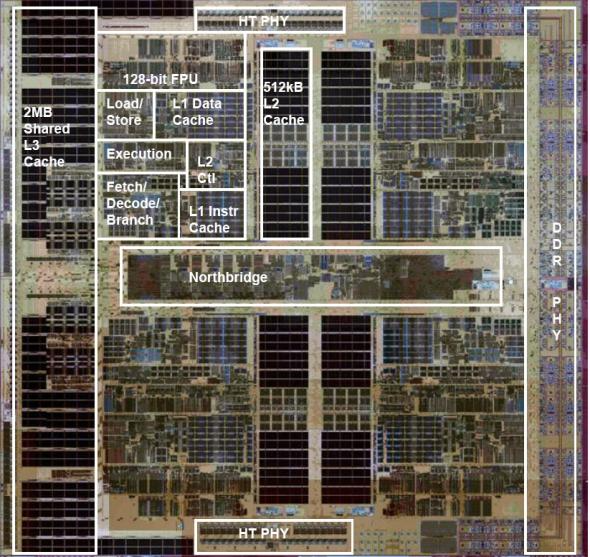
\includegraphics[scale=0.4]{images/amd_barcelona_die.png}
\end{center}

\section{Instructions: Language of the Computer}

To command a computer you must speak its language. The words of a computer language are called \textit{instructions}, and its vocabulary called an \textit{instruction set}. The \textit{stored-program concept} is the idea that instructions and data of many types can be stored in a computer's memory as numbers.

\subsection{Instructions for Making Decisions}

\textit{Conditional branch} instructions are analogous to \verb|if| and \verb|goto| statements in a programming language e.g. the following ``branch if equal'' instruction
\begin{center}
    \verb|beq register1, register2, L1|
\end{center}
goes to the statement labeled \verb|L1| if the value in \verb|register1| and \verb|register2| are equal.


\section{Arithmetic for Computers}

Addition, substraction, multiplication, division, floating point, ALU, etc.

\section{The Processor}

To understand the basics of a processor implementation, we can look at the construction of the datapath and control path for an implementation of the MIPS instruction set. This includes a subset of the core MIPS instruction set:
\begin{itemize}
    \item The memory reference instructions load word (\verb|lw|) and store word (\verb|sw|)
    \item The arithmetic-logical instructions \verb|add|,\verb|sub|,\verb|AND|,\verb|OR|, and \verb|slt|
    \item The instructions branch equal (\verb|beq|) and jump(\verb|j|)
\end{itemize}

Overall, much of what needs to be done to implement these instructions is the same regardless of the exact class of instruction. For every instruction, the first two steps are identical:
\begin{enumerate}
    \item Send the program counter (PC) to the memory that contains the code and fetch the instruction from that memory.
    \item Read one or two registers, using fields of the instruction to select the registers to read. 
\end{enumerate}
For example, the diagram below shows a high level, abstract outline of a MIPS processor implementation.
\begin{center}
    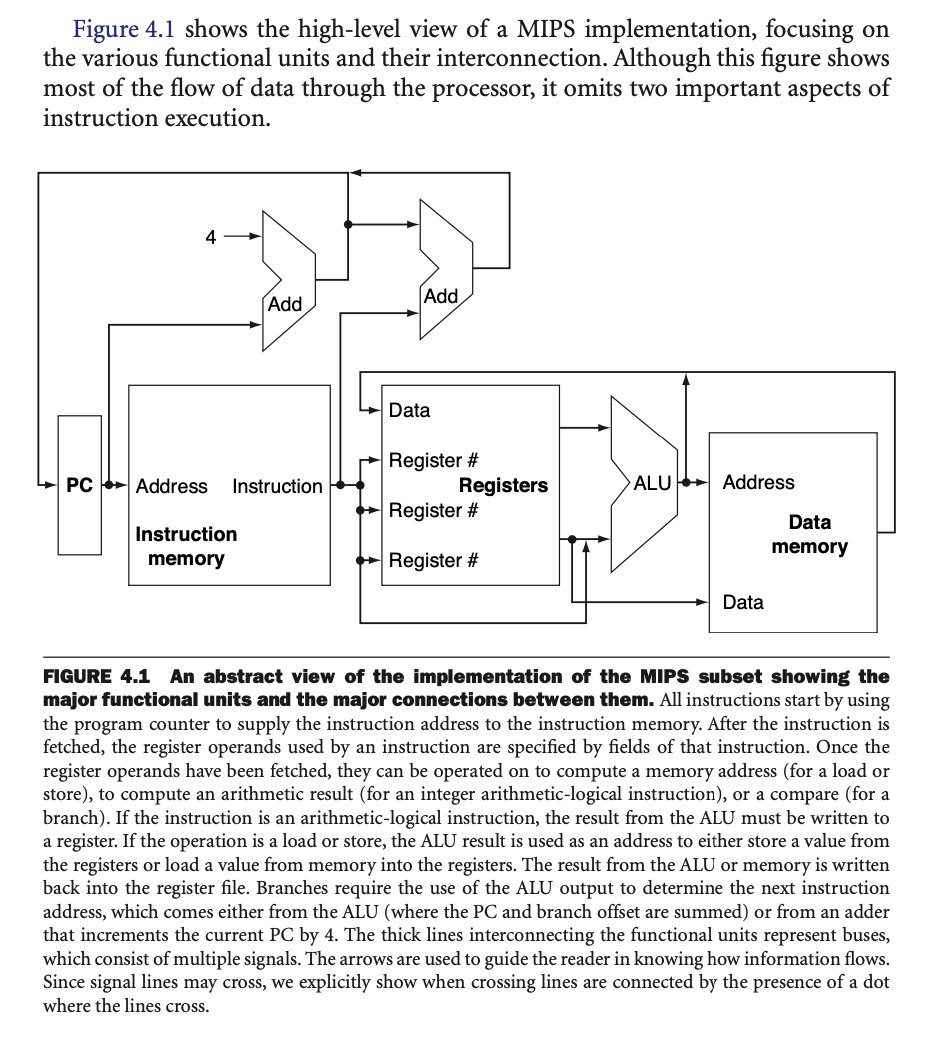
\includegraphics[scale=0.45]{images/mips_processor_high_level.png}
\end{center}

\subsection{Logic Design Conventions}

Note that the datapath elements of a MIPS implementation consists of two different type of logic elements:
\begin{itemize}
    \item \textbf{Combinational}: elements that operate on data values, where their outputs always depend only on the current inputs (i.e. think of them as implementing pure functions)
    \item \textbf{Sequential}: elements that contain some internal \textit{state}. These elements have at least two inputs and one output, where the inputs are:
    \begin{enumerate}
        \item The data value to be written.
        \item The clock.
    \end{enumerate}
    The output from a sequential logic component provides the value that was written in an earlier clock cycle.
\end{itemize}
A \textit{clocking methodology} defines when signals can be read and when they can be written. We can assume an \textit{edge-triggered clocking} methodology, which means that any values stored in a sequential logic element are updated only on a clock edge. 

Since state (i.e. sequential) elements are the only ones that can store values, any collection of combinational logic must have its inputs come from a set of state elements and its outputs written into a set of state elements The inputs are values that were written in a previous clock cycle, while the outputs are values that can be used in a following clock cycle.

\subsection{Pipelining}

MIPS instruction execution classically takes five steps:
\begin{enumerate}
    \item \textbf{Fetch} instruction from memory.
    \item \textbf{Read} registers while \textbf{decoding} the instruction.
    \item \textbf{Execute} the operation to calculate an address.
    \item Access an operand in data \textbf{memory}.
    \item \textbf{Write} the result into a register.
\end{enumerate}

\section{The Memory Hierarchy}

In an ideal world, we would have an infinitely large and fast memory for our computer, but this is not feasible in practice, since fast memory is costly. So, instead, we simulate the illusion of an infinite memory by using a \textit{memory hierarchy}. That is, a progressively larger and slower series of caches that serve as memory for the processor.
\begin{center}
    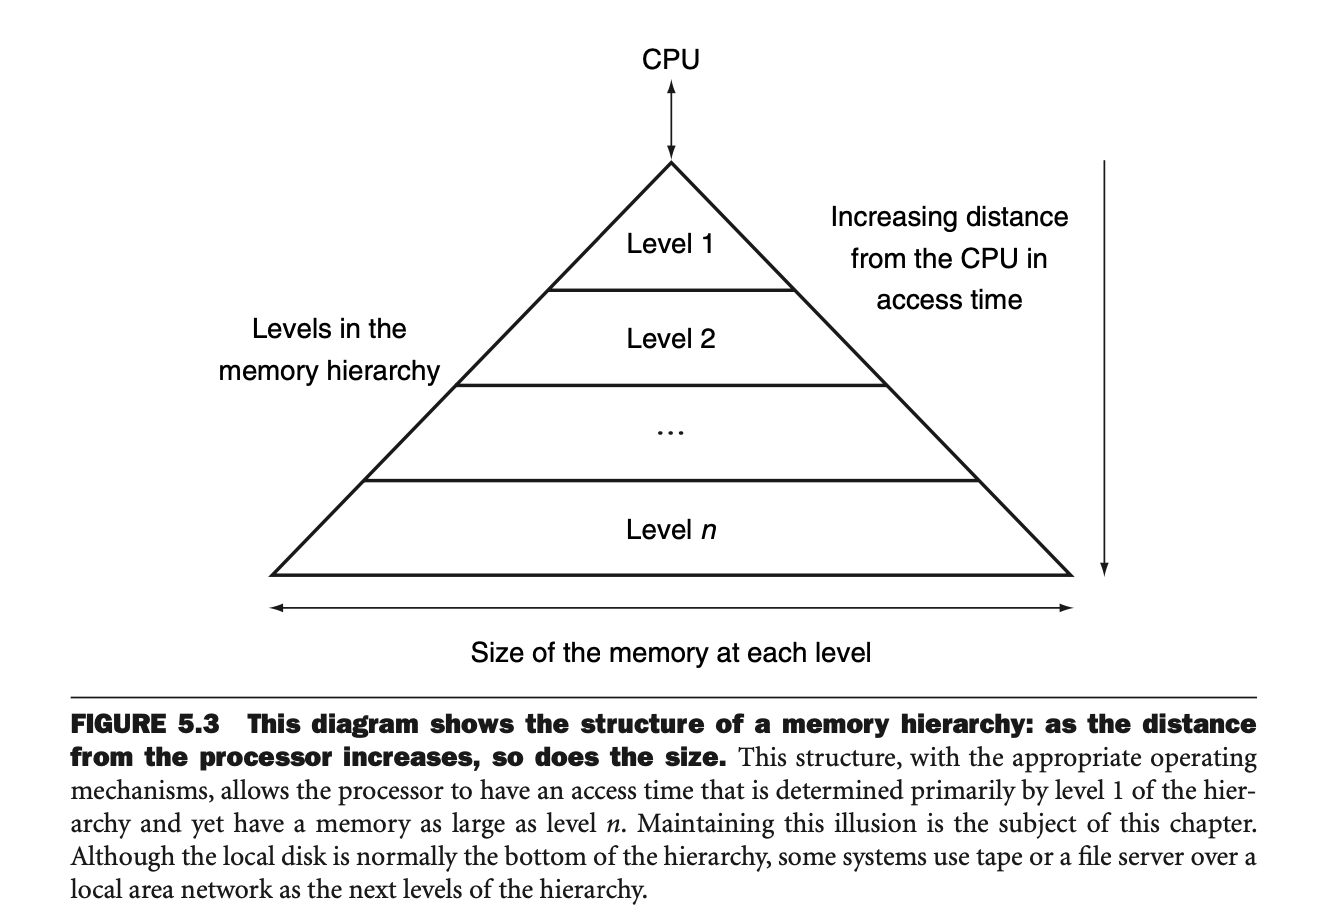
\includegraphics[scale=0.35]{images/memory_levels.png}
\end{center}
Note that the \textit{principle of locality} underlies the way that programs operate. That is, the assumption is that programs access a relatively small portion of their address space at any instant of time. There are two different types of locality:
\begin{itemize}
    \item \textbf{Temporal locality}: if an item is referenced at some point in time, it is likely to be referenced again soon.
    \item \textbf{Spatial locality}: if an item is referenced, other items that are nearby are likely to be referenced soon.
\end{itemize}
We make use of this to construct the memory hierarchy from a series of \textit{caches}, that get progressively faster and smaller as they get closer to the actual processor.

A memory hierarchy may consist of multiple levels, but data is copied only between two adjacent levels at a time, so we can consider only two levels when describing the caching mechanisms. There is an \textit{upper level} (faster and closer to the processor) and a \textit{lower level}. The smallest unit of information that can be either present or absent from any cache level is typically referred to as a cache \textit{block} or \textit{line}.

\begin{center}
    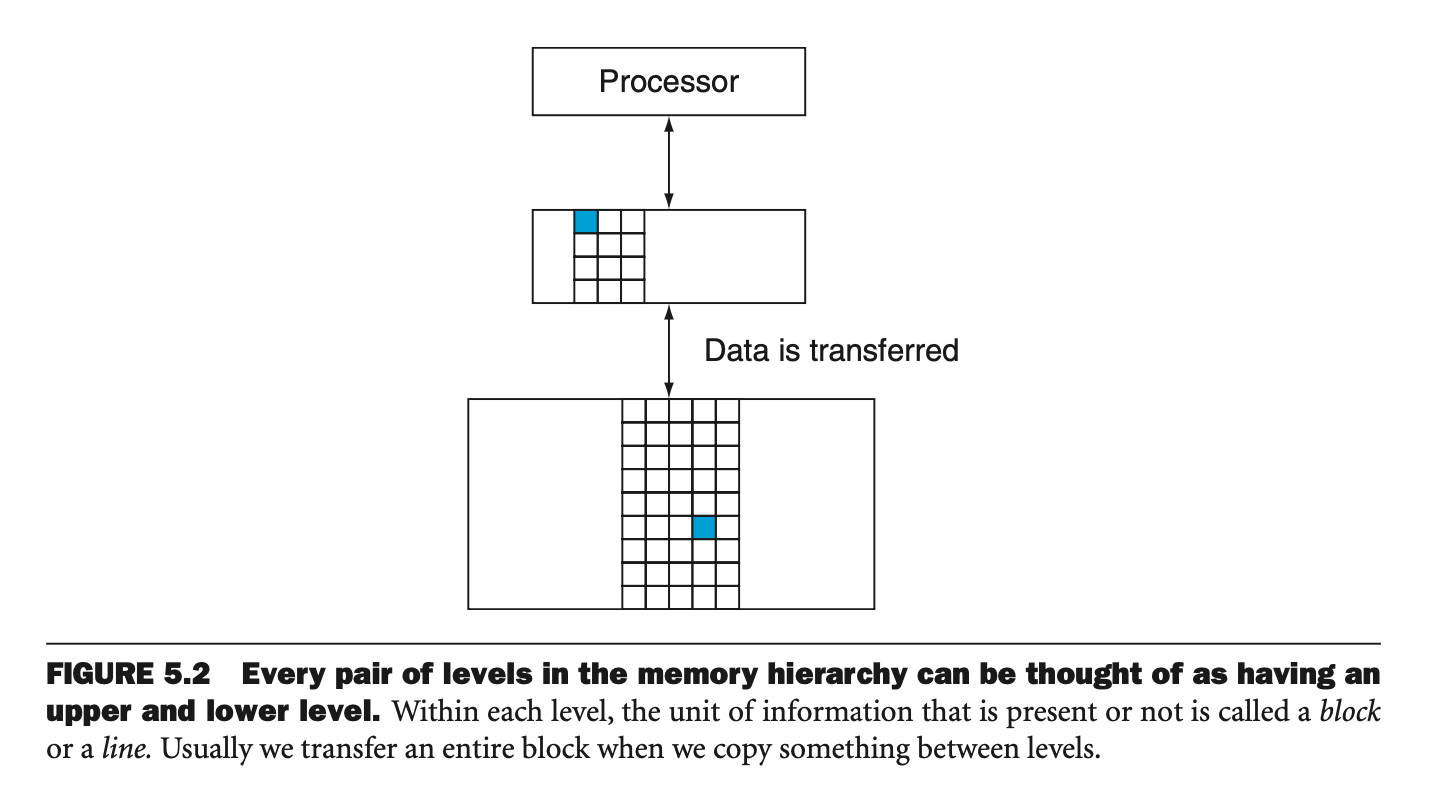
\includegraphics[scale=0.35]{images/mem_2levels.png}
\end{center}

\subsection{Cache Basics}

In a basic scenario, we can imagine that a processor issues memory requests that are each one word (e.g. 32 bits) and the blocks in the cache are also one word. If a cache contains words $X_1,\dots,X_{n-1}$ prior to a request for a word $X_n$ not in the cache, then a cache miss occurs and $X_n$ is brought into the cache.

When servicing a processor request, we need to know (1) is the data item in the cache and, if so, (2) how do we find it? The simplest approach is to simply map each word to a locatino in the cache based on its address, which is known as \textit{direct mapping}. This is essentially a simple hash based addressing scheme. With this approach, however, there may be collisions in addresses that map to the same cache location, so we need to deal with this. One approach is to add a set of \textit{tags} to the cache. Basically, for each cache entry, we add a tag that contains the bits of the address that were not included in the hash function, so that we can disambiguate between two addresses that may map to the same cache location. In practice we may also include a \textit{valid} bit that tells whether a particular cached value is currently valid to use or not.

\subsubsection*{Set Associative Caches}

An alternative to the direct mapping approach is to make the cache \textit{set associative}. So, instead of giving every address exactly one location in the cache, we give it $n$ possible locations, which we call $n$-way set associative. If the cache can hold $m$ entries then a $m$-way set associative cache is also referred to as \textit{fully associative}. In this other extreme, it means that a block can be placed anywhere in the cache, but then comes with the tradeoff that finding a block is more expensive, since we may need to search through every block to find it.
\begin{center}
    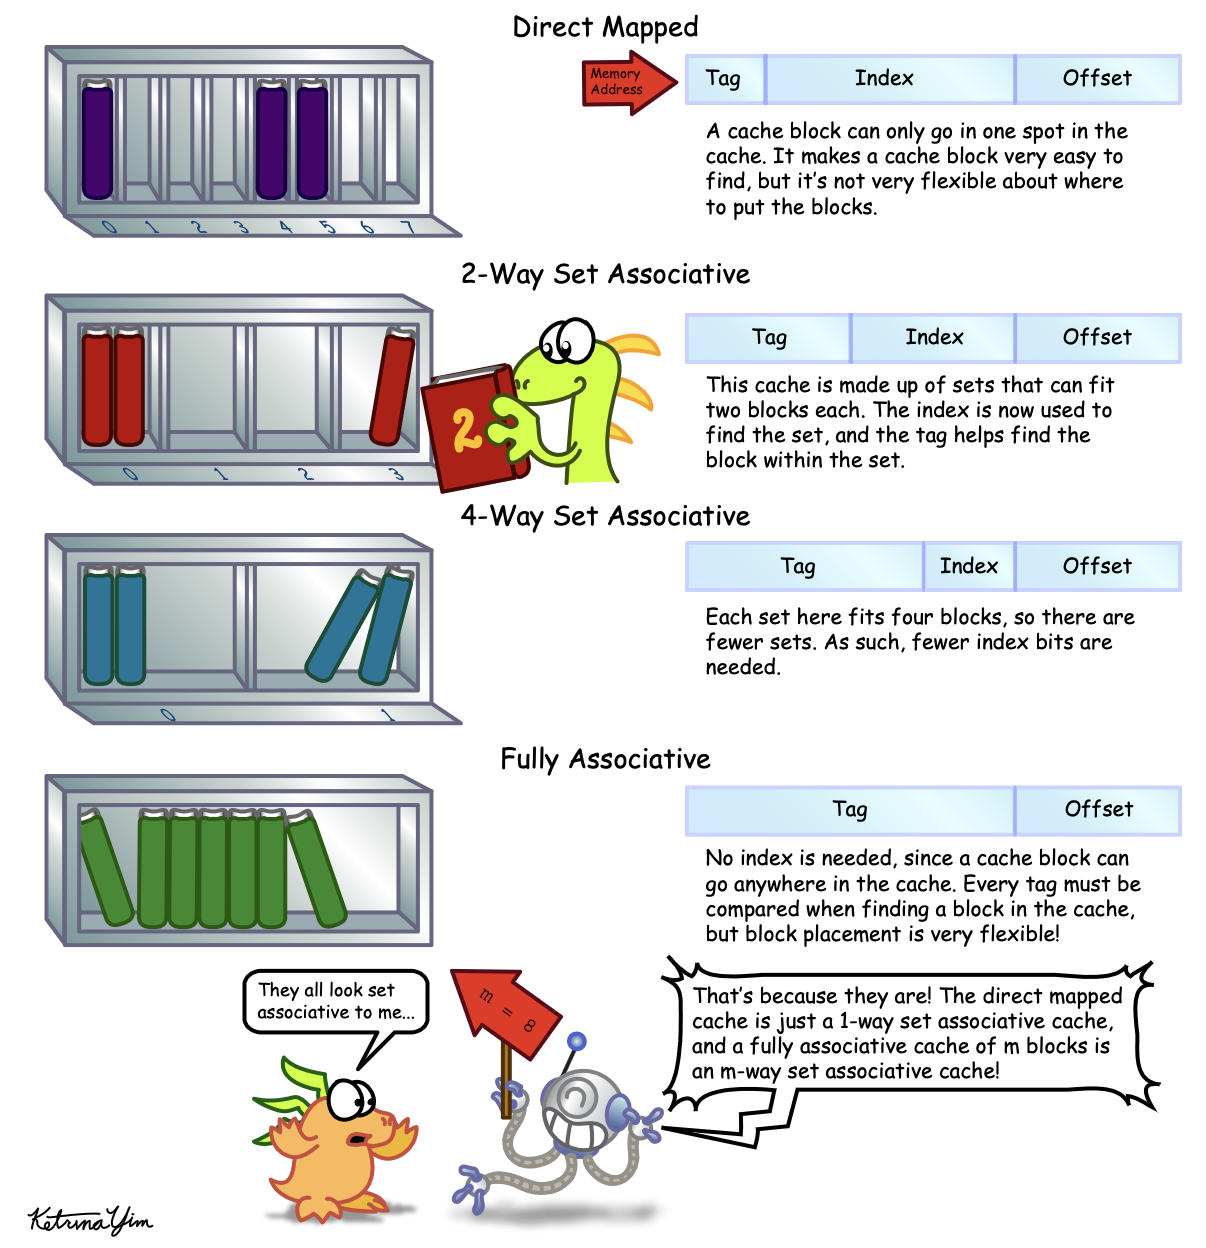
\includegraphics[scale=0.35]{images/cache_assoc.png}
\end{center}
Note that allowing for more potential locations for a block can decrease contention for blocks, since if there are only a few unused blocks, a new request is then free to pick any unused block. This is in contrast to a direct mapped scheme, where choice of block is completely determined by the address mapping function. Also, in an associative cache, we have a choice of where to place the new block, so potentially a choice of which block to kick out of the cache. The most commonly used scheme is \textit{least recently used} (LRU) i.e. we remove blocks that were unused for the longest time.

\section{Hardware Description Languages}


\textit{Hardware description languages (HDLs)} are languages for describing digital circuits at a higher level of abstraction, rather than directly describing every logic gate and their exact placement, connections, etc. 

\subsection*{Verilog}

\textit{Verilog} is one of the most common HDLs, and it can be used to define both combinational and sequential circuits. As a simple example, we can describe a simple combinational circuit in Verilog as a \textit{module}. For example, the following describes a circuit with one \textit{input} and one \textit{output}, where the output is the negation of the input.
\begin{verbatim}
    module top_module(input a, output b);
        assign b = !a;
    endmodule
\end{verbatim}
When circuits become more complex, we can also declare \textit{wires}, which are like internal connections that are not externally visible outside of the module. For example, the following declares an internal wire that takes on the negation of the input \verb|a|, and this wire is then fed (i.e. connected to) the output. For this simple example the wire doesn't really serve a necessary purpose, but with larger circuits wires can help to decompose more complex bits of logic.
\begin{verbatim}
    module top_module(input a, output b);
        wire w1; // wire declaration.
        assign w1 = !a;
        assign b = w1;
    endmodule
\end{verbatim}

\bibliographystyle{plain}
\bibliography{../../references.bib}

\end{document}